\section{Framebuffer 與輸出實作細節}
\label{app:framebuffer-details}

\subsection{座標與 Pixel Row}

UI、滑鼠與 Scene 都採左上角原點、Y 軸向下；OpenGL framebuffer 則以左下角為原點，pixel rows 也由下往上排列。擷取 UI 區域時，程式以視窗高度、區域上緣與區域高度換算 \lstinline|glReadPixels()| 使用的 bottom 座標。這個換算只改變讀取位置，不會翻轉讀回的資料。

\begin{figure}[tbp]
    \centering
    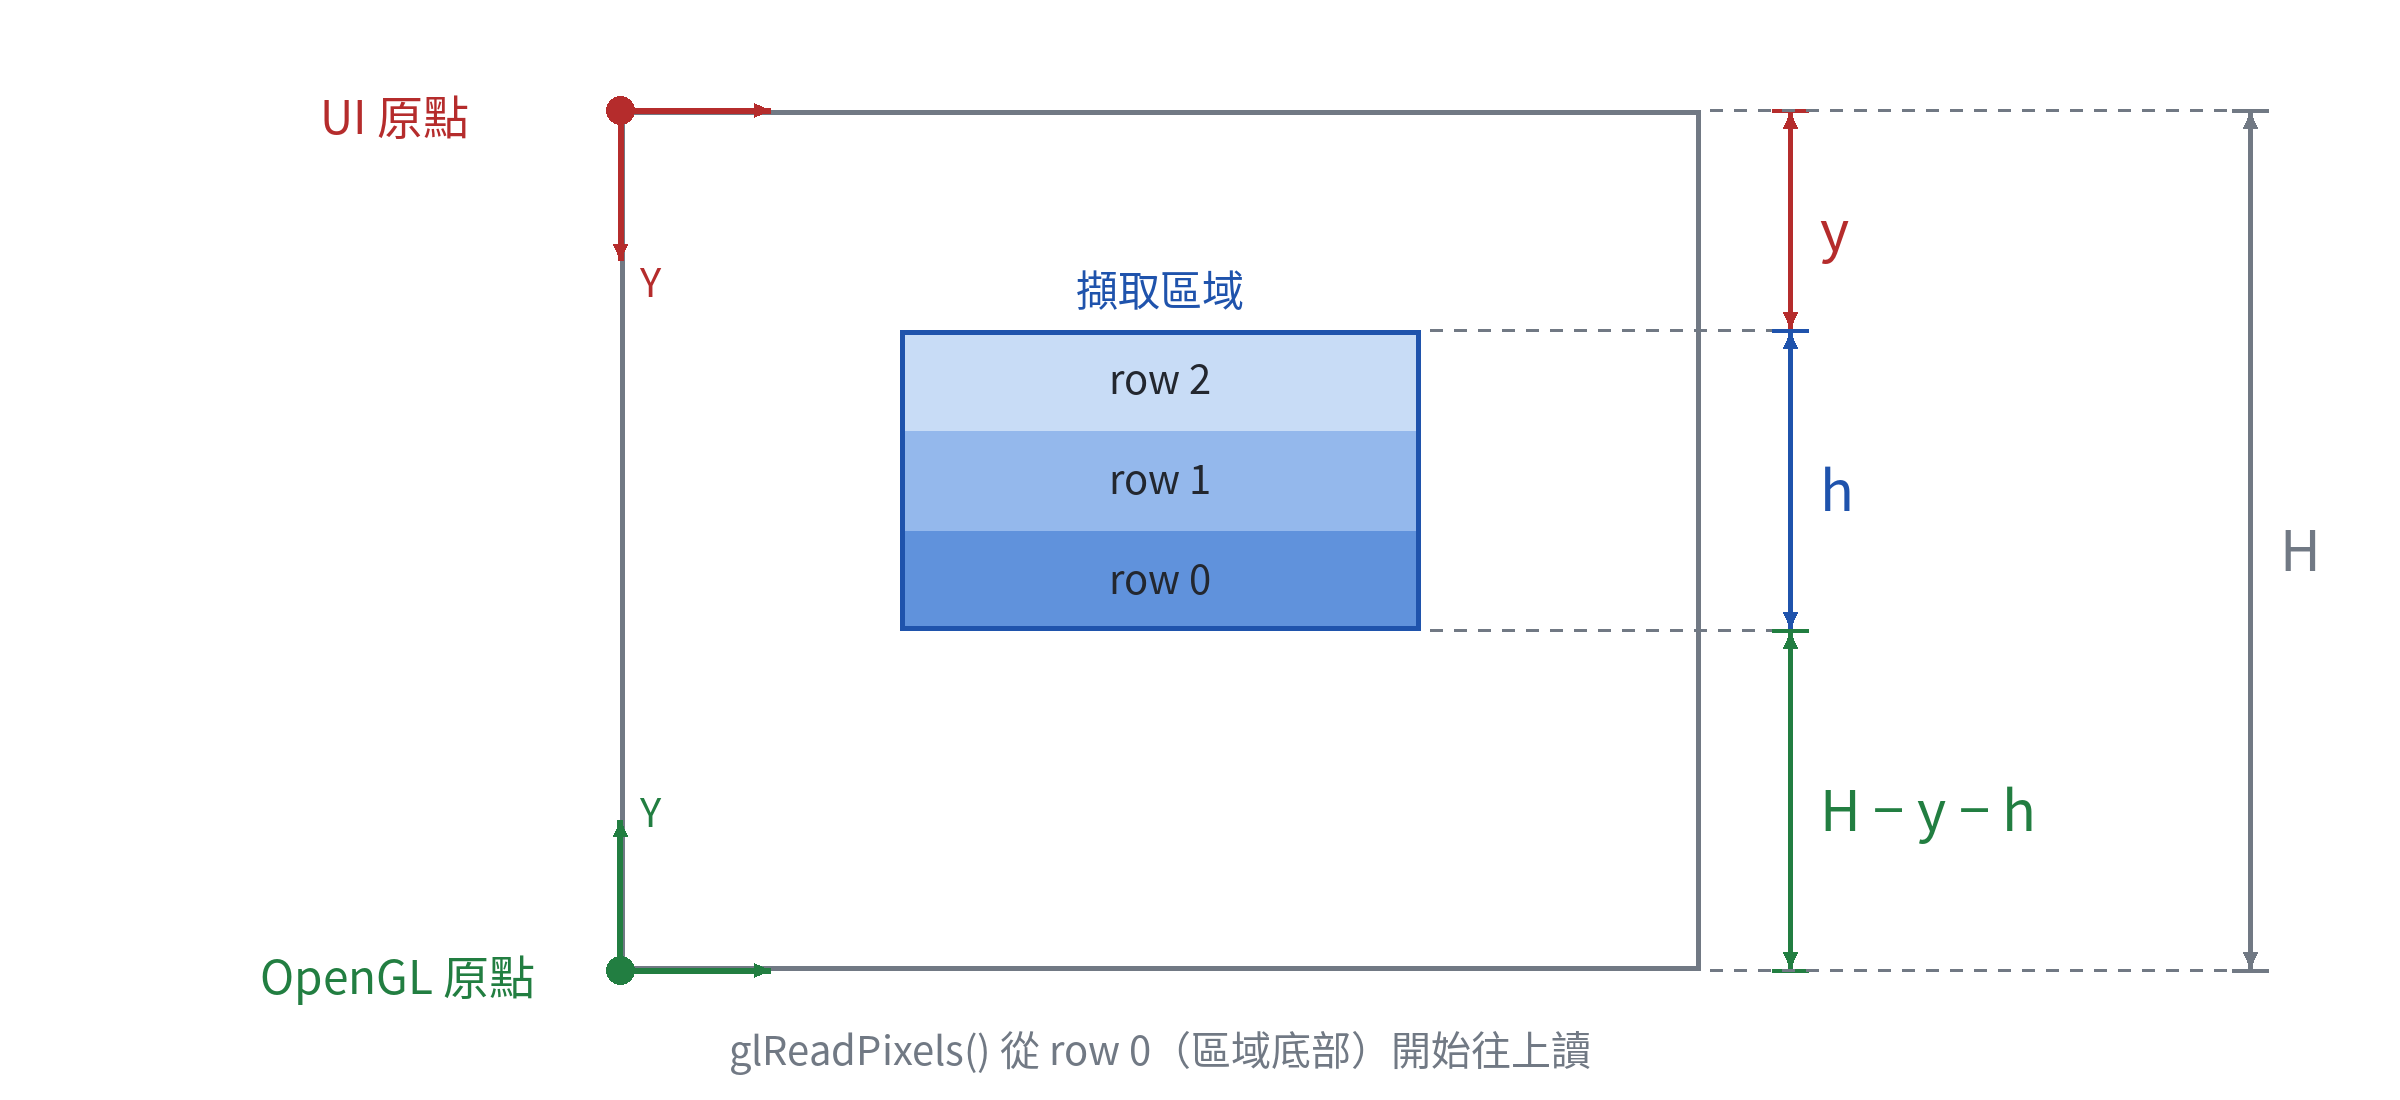
\includegraphics[width=.92\textwidth]{docs/figures/ch06_framebuffer-coordinate.png}
    \caption{UI 與 OpenGL framebuffer 的座標及 pixel row 順序}
    \label{fig:framebuffer-coordinate}
\end{figure}

\subsection{擷取與還原狀態}

程式從 single-buffer 的 front buffer 擷取像素。還原前會暫時關閉 blending、depth、stencil、scissor 與 alpha test，並在操作完成後恢復 PACK／UNPACK alignment 與其他 OpenGL state，避免 ColorBuffer 影響後續 Renderer。Timer 擷取多視窗內容時也會先切換到目標 GLUT window，完成後只在原 window ID 仍有效時切回。

\subsection{PPM P6 轉換}

PpmExporter 由 \lstinline|height - 1| 反向走訪到第 0 列，將 framebuffer 的 bottom-up RGBA 資料轉成 PPM 所需的 top-down RGB bytes，alpha channel 不輸出。圖~\ref{fig:ppm-export-layout} 顯示 row order、header 與 channel 配置。

\begin{figure}[tbp]
    \centering
    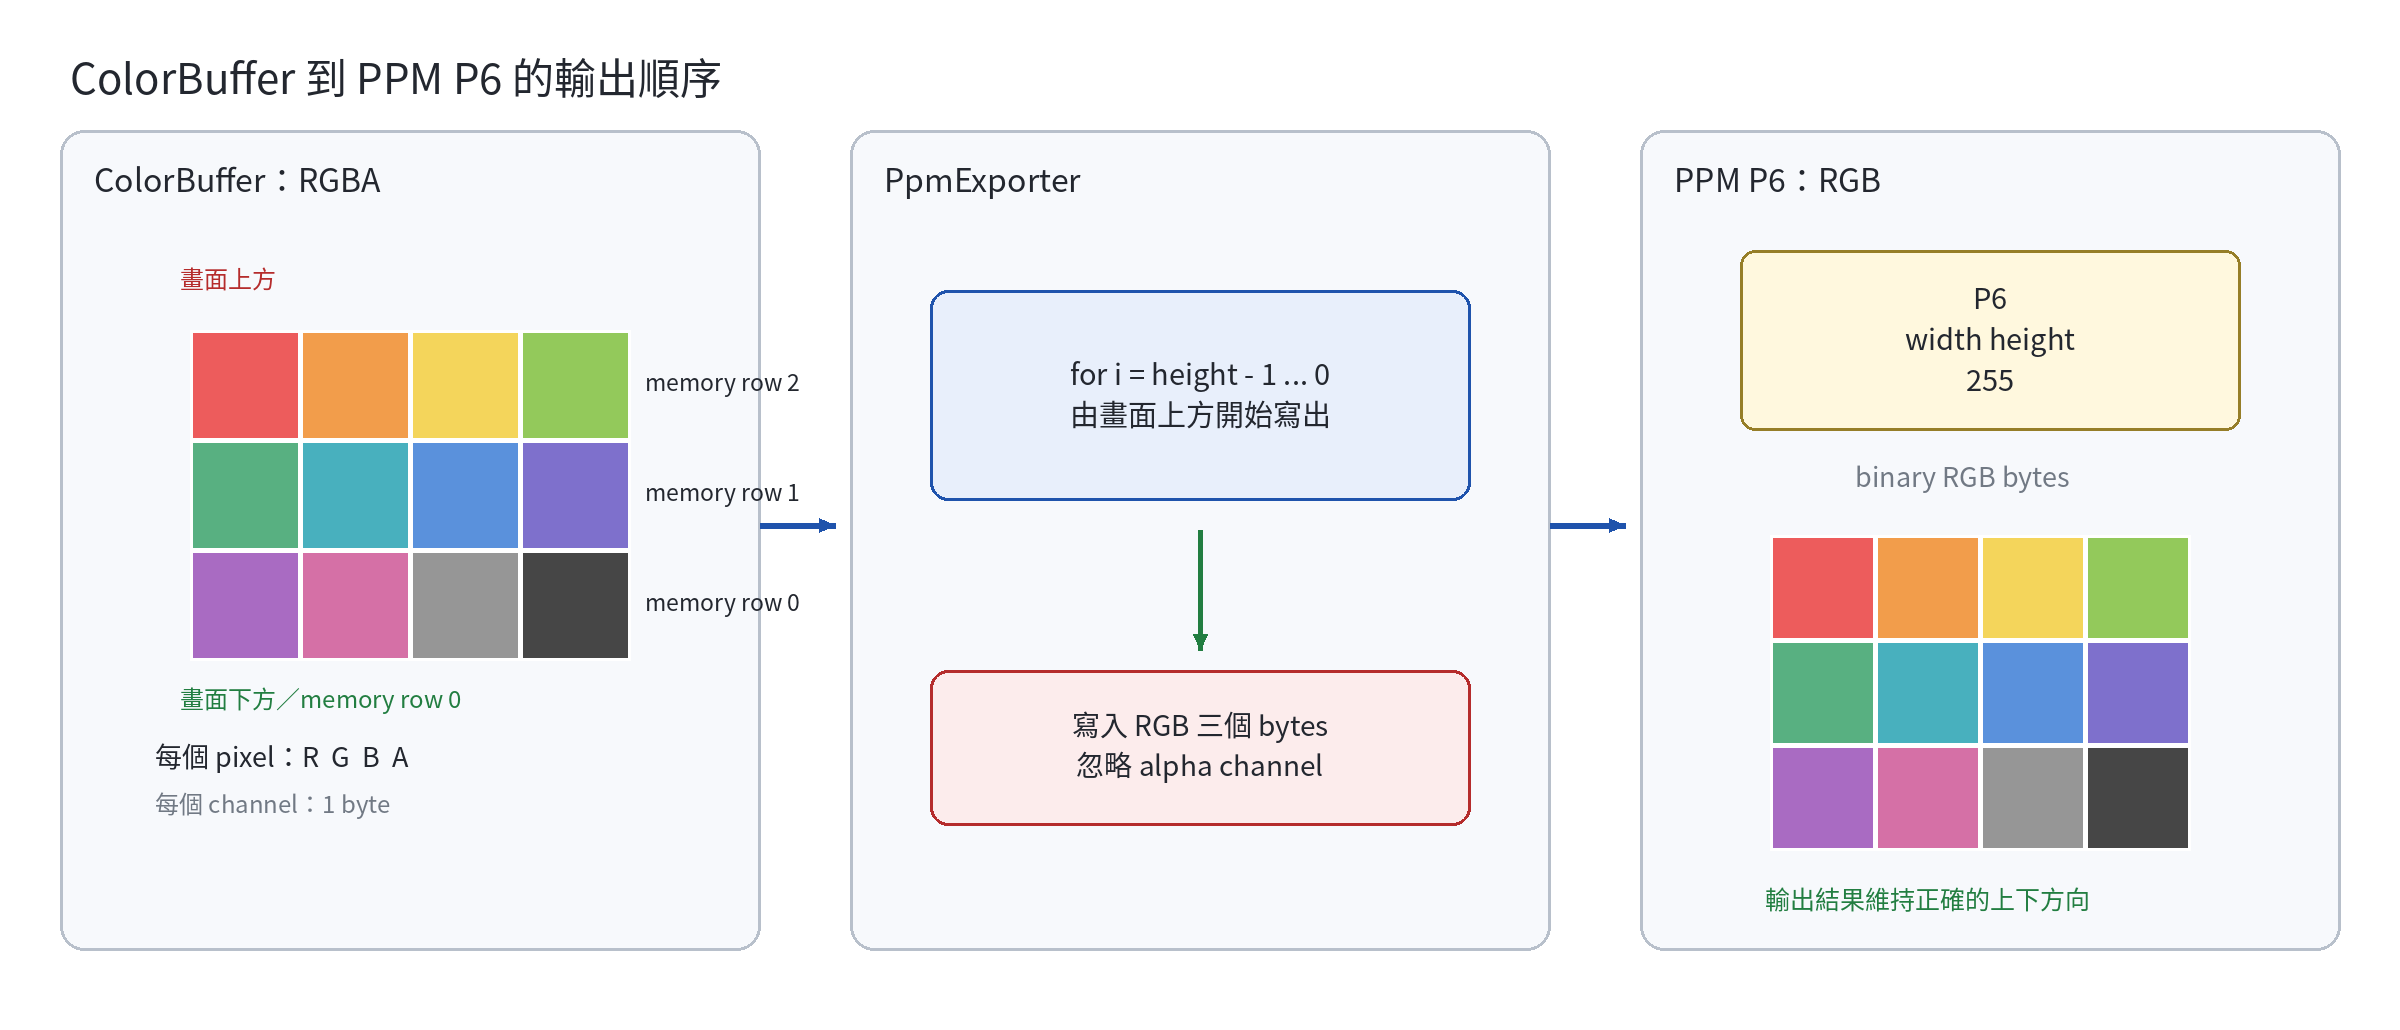
\includegraphics[width=.92\textwidth]{docs/figures/ch06_ppm-export-layout.png}
    \caption{ColorBuffer 轉成 PPM P6 時的列順序與 channel 配置}
    \label{fig:ppm-export-layout}
\end{figure}
